% Ortskurve Zweipol-Admittanz
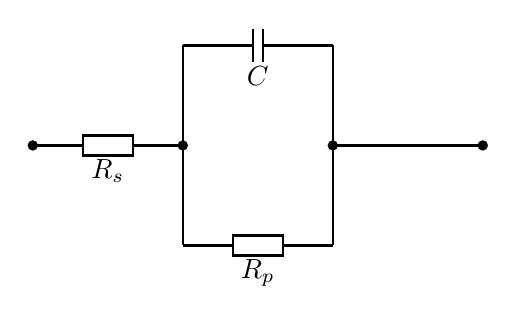
\begin{tikzpicture}[scale=2.54]%
% dpic version 2024.01.01 option -g for TikZ and PGF 1.01
\ifx\dpiclw\undefined\newdimen\dpiclw\fi
\global\def\dpicdraw{\draw[line width=\dpiclw]}
\global\def\dpicstop{;}
\dpiclw=0.8bp
\dpiclw=0.8bp
\dpicdraw[fill=black](0,0) circle (0.007874in)\dpicstop
\dpicdraw (0,0)
 --(0.25,0)\dpicstop
\dpicdraw (0.5,0)
 --(0.5,0.05)
 --(0.25,0.05)
 --(0.25,-0.05)
 --(0.5,-0.05)
 --(0.5,0)\dpicstop
\dpicdraw (0.5,0)
 --(0.75,0)\dpicstop
\draw (0.375,-0.05) node[below=-2bp]{$ R_s$};
\dpicdraw[fill=black](0.75,0) circle (0.007874in)\dpicstop
\dpicdraw (0.75,0)
 --(0.75,0.5)\dpicstop
\dpicdraw (0.75,0.5)
 --(1.1,0.5)\dpicstop
\dpicdraw (1.1,0.416667)
 --(1.1,0.583333)\dpicstop
\dpicdraw (1.15,0.416667)
 --(1.15,0.583333)\dpicstop
\dpicdraw (1.15,0.5)
 --(1.5,0.5)\dpicstop
\draw (1.125,0.416667) node[below=-2bp]{$ C$};
\dpicdraw (1.5,0.5)
 --(1.5,0)
 --(2.25,0)\dpicstop
\dpicdraw[fill=black](2.25,0) circle (0.007874in)\dpicstop
\dpicdraw (0.75,0)
 --(0.75,-0.5)\dpicstop
\dpicdraw (0.75,-0.5)
 --(1,-0.5)\dpicstop
\dpicdraw (1.25,-0.5)
 --(1.25,-0.45)
 --(1,-0.45)
 --(1,-0.55)
 --(1.25,-0.55)
 --(1.25,-0.5)\dpicstop
\dpicdraw (1.25,-0.5)
 --(1.5,-0.5)\dpicstop
\draw (1.125,-0.55) node[below=-2bp]{$ R_p$};
\dpicdraw (1.5,-0.5)
 --(1.5,0)\dpicstop
\dpicdraw[fill=black](1.5,0) circle (0.007874in)\dpicstop
\end{tikzpicture}%
